\section{Uniform thinness and the Cayley graph}
\label{sec:geometry-thinness}

We complete the hyperbolicity assertion of
Theorem~\ref{thm:triangle-complex}. Throughout this section the triangulation
of $K$ is its fixed barycentric subdivision. Thus every model triangle
contains an original vertex of $K$. A reduced diagram means a diagram from
Lemma~\ref{lem:reduced-diagrams} over this fixed triangulation. Its metric
$d_\Delta$ is the intrinsic piecewise Euclidean metric of the whole
diagram. At every interior vertex its total angle is at least $2\pi$;
at one mapping to an original vertex of $K$ it is at least $2\pi+\eta$.
The number $\eta>0$ is fixed independently of the diagram.

The strict angle excess has a uniform metric effect because each small
triangle contains an original vertex. Angular Gauss--Bonnet bounds the
number of these vertices inside a simple geodesic polygon, and the fixed
mesh then bounds its inradius. A level-arc argument converts that bound
to thinness. We subsequently compare controlled paths with geodesics and
apply the comparison to expanded Cayley-graph sides.

\subsection{Angle excess and thin diagrams}

\begin{lemma}[Uniform thinness of reduced diagrams]
\label{lem:diagram-thinness}
Choose $M>0$ larger than every diameter and edge length among the finitely
many model triangles and edges. Put
\[
 A=M+\frac{2M\pi}{\eta},\qquad \delta=10(A+1).
\]
Every geodesic triangle in every reduced diagram is $\delta$-thin.
\end{lemma}

\begin{proof}
We isolate a simple geodesic polygon, use angle excess and the fixed
barycentric mesh to bound distance to its boundary, and then use a level
arc to bound distance from one side to the others.

Fix a point $p$ of one geodesic side. If $p$ belongs to either other side,
there is nothing to prove. Otherwise let $(a,b)$ be the component of this
side outside the union of the other two sides which contains $p$.
The endpoints exist since the endpoints of the entire side lie on that
union. There is a simple path $Q$ from $a$ to $b$ on the other sides
consisting of at most two geodesic subarcs. If one side contains both
$a$ and $b$, use its subarc. In the remaining case write the other sides
as $\alpha,\beta$, with $a\in\alpha$, $b\in\beta$, and common corner $c$.
Follow $\alpha[a,c]$ to its first meeting $w$ with the compact arc
$\beta[b,c]$, and use
$\alpha[a,w]\cup\beta[w,b]$. The first-meeting condition makes the two
interiors disjoint, irrespective of any later intersections of
$\alpha$ and $\beta$. The interior of $[a,b]$ misses $Q$ by its definition.

Consequently $[a,b]\cup Q$ is a simple closed curve with at most three
geodesic sides. It bounds a disk $\Omega\subset\Delta$: an omitted point
inside this curve would belong to a bounded complementary component of
the planar diagram, contrary to its having no holes. By
Lemma~\ref{lem:finite-geodesics}, the sides have finitely many straight
pieces. Insert these pieces in the diagram, subdivide at their
intersections with its edges, and triangulate the resulting pieces of
$\Omega$.

Let $n$ count the diagram vertices in $\Omega^\circ$ mapping to original
vertices of $K$. At every such vertex all its diagram sectors are present
in $\Omega$: a planar neighborhood of an interior point of the Jordan
disk is contained in that disk. Its angle therefore has the full excess
of at least $\eta$. Other interior vertices have angle at least $2\pi$;
newly inserted ones have angle exactly $2\pi$. At a boundary vertex
other than the at most three corners, the angle on the inside is at least
$\pi$, since a smaller angle would give a local shortcut to the geodesic
side. Each corner has boundary deficit at most $\pi$. Applying
\eqref{eq:gauss-bonnet} to this disk gives
\[
 2\pi\le 3\pi-n\eta,\qquad n\le\frac{\pi}{\eta}.
\]

We first bound the distance to the polygon boundary. All distances here
and below are $d_\Delta$, even when minimizing routes leave $\Omega$.
Set $f(x)=d_\Delta(x,\partial\Omega)$.
For an interior point $x$, choose a closed triangle of the fixed
barycentric diagram containing $x$, before the auxiliary subdivision
along the polygon boundary. Join $x$ inside it to its vertex mapping
to an original vertex of $K$; the segment has length less than $M$.
Either this segment first meets $\partial\Omega$, in which case
$f(x)<M$, or it ends at one of the $n$ vertices just counted. Thus every
point with $f(x)>M$ lies in an ambient ball of radius $M$ about one of
those vertices. Since $f$ is $1$-Lipschitz, each such ball contributes
values in an interval of length $2M$. The continuous function $f$ on the
connected compact disk takes every value from $0$ to its maximum $F$.
If $F>M$, the interval $(M,F]$ is therefore covered by $n$ intervals of
total length at most $2Mn$. Hence
\begin{equation}
 d_\Delta(x,\partial\Omega)\le M+2Mn\le A
 \quad (x\in\Omega).
 \label{eq:polygon-inradius}
\end{equation}
The segments used in this argument are actual paths in $\Delta$;
allowing additional routes outside $\Omega$ only decreases the distances.

Suppose now that $R=d_\Delta(p,Q)>10(A+1)$. On a sufficiently fine
Euclidean subdivision of $\Omega$, interpolate the values of
$d_\Delta(p,\cdot)$ linearly at the vertices to obtain a continuous
piecewise linear function $h$ with
\[
 |h(x)-d_\Delta(p,x)|<1.
\]
Include $p$ and all side breakpoints among the subdivision vertices.
On $[a,b]$ the interpolant agrees exactly with distance to $p$, since
that side is geodesic and its distance function is linear on each side
of $p$. On $Q$ we have $h\ge R-1$. Choose
$t\in(R/3,2R/3)$ different from all vertex values of $h$.
Because $a,b\in Q$, both distances $d_\Delta(p,a)$ and
$d_\Delta(p,b)$ are at least $R$. Thus the level $h=t$ has exactly two
boundary endpoints, both on $[a,b]$, one on each side of $p$, and no
endpoint on $Q$.

Inside each small triangle the level consists of a segment or is empty;
segments join in pairs across interior edges. A component with a boundary
endpoint must therefore be an arc, and the two boundary endpoints must
belong to the same component. Call that arc $\gamma$. For $y\in\gamma$,
\[
 \frac R3-1<d_\Delta(p,y)<\frac{2R}3+1,
 \qquad
 d_\Delta(y,Q)\ge R-d_\Delta(p,y)>\frac R3-1>A.
\]
By \eqref{eq:polygon-inradius}, a nearest boundary point to $y$ is
therefore on $[a,b]$ and is at distance at most $A$.
At the two endpoints of $\gamma$, the values of
$d_\Delta(a,\cdot)$ lie on opposite sides of $d_\Delta(a,p)$.
The intermediate value theorem supplies $y\in\gamma$ such that
$d_\Delta(a,y)=d_\Delta(a,p)$. Choose $z\in[a,b]$ with
$d_\Delta(y,z)\le A$. Figure~\ref{fig:level-arc} records the
topological configuration. Since $[a,b]$ is geodesic,
\[
 d_\Delta(z,p)
 =\bigl|d_\Delta(a,z)-d_\Delta(a,p)\bigr|
 =\bigl|d_\Delta(a,z)-d_\Delta(a,y)\bigr|\le A.
\]
It follows that $d_\Delta(p,y)\le2A$, whereas
$d_\Delta(p,y)>R/3-1>2A$. This contradiction proves
$d_\Delta(p,Q)\le\delta$. Since $Q$ lies on the other two sides, it
proves the lemma.
\end{proof}

\begin{figure}[htbp]
\centering
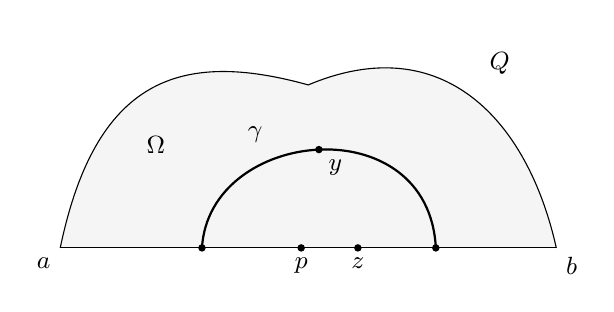
\begin{tikzpicture}[scale=.9, every node/.style={font=\small}]
  \coordinate (a) at (-3.5,0);
  \coordinate (b) at (3.5,0);
  \coordinate (p) at (-.1,0);
  \coordinate (z) at (.7,0);
  \coordinate (y) at (.15,1.3875);
  \fill[gray!8] (a)
    .. controls (-3,2.4) and (-1.8,2.8) .. (0,2.3)
    .. controls (1.9,3.1) and (3.1,1.8) .. (b)--cycle;
  \draw (a)--(b);
  \draw (a)
    .. controls (-3,2.4) and (-1.8,2.8) .. (0,2.3)
    .. controls (1.9,3.1) and (3.1,1.8) .. (b);
  \draw[thick] (-1.5,0)
    .. controls (-1.4,1.7) and (1.7,2) .. (1.8,0);
  \fill (-1.5,0) circle (1.5pt);
  \fill (1.8,0) circle (1.5pt);
  \fill (p) circle (1.5pt);
  \fill (z) circle (1.5pt);
  \fill (y) circle (1.5pt);
  \node[below left] at (a) {$a$};
  \node[below right] at (b) {$b$};
  \node[below] at (p) {$p$};
  \node[below] at (z) {$z$};
  \node[below right] at (y) {$y$};
  \node at (-.75,1.6) {$\gamma$};
  \node at (-2.15,1.45) {$\Omega$};
  \node at (2.7,2.6) {$Q$};
\end{tikzpicture}
\caption{The auxiliary Jordan disk and the level arc $\gamma$. The two
endpoints of $\gamma$ lie on $[a,b]$, on opposite sides of $p$;
$y$ and $z$ are the points selected in the proof. Only topological
incidences are shown. Distances are measured in the whole diagram;
shortest routes may leave $\Omega$ and are not drawn.}
\label{fig:level-arc}
\end{figure}

\subsection{Stability of controlled paths}

The next statement is the form of the classical Morse stability lemma
\cite[Chapter~III.H, Theorem~1.7, p.~401]{BH1999} needed to pass from diagram distances to
word distances. We include its
proof with constants suited to the present application. In its hypothesis, a subarc means a parameter
subinterval of the path; repetitions and retracing are allowed.

\begin{lemma}[Stability of paths with controlled subarc lengths]
\label{lem:path-stability}
Let $X$ be a geodesic metric space with $\delta$-thin geodesic triangles.
Fix $\lambda\ge1$ and $C\ge0$. There is $D=D(\delta,\lambda,C)$ such that
every rectifiable path $\sigma$ satisfying
\begin{equation}
 \operatorname{length}(\sigma|_{[u,v]})
 \le\lambda d(\sigma(u),\sigma(v))+C
 \quad\text{for every }u\le v
 \label{eq:all-subarc-bound}
\end{equation}
lies in the $D$-neighborhood of a geodesic $J$ with the same endpoints,
and $J$ lies in the $2D$-neighborhood of $\sigma$.
Consequently triangles whose three sides satisfy
\eqref{eq:all-subarc-bound} are $(3D+\delta)$-thin.
\end{lemma}

\begin{proof}
A point has a nearest point on $J$, because a geodesic segment is compact.
We first prove a projection estimate. Suppose $R_0>4\delta$,
$d(x,J),d(y,J)\ge R_0$, and $d(x,y)\le R_0/2$. Choose nearest points
$x',y'\in J$. Every point $z\in[x',y']\subset J$ is within $2\delta$
of one of the other three sides of the geodesic quadrilateral
$x,x',y',y$; a diagonal reduces this assertion to two thin triangles.
It cannot be within $2\delta$ of $w\in[x,y]$, for then
\[
 R_0\le d(x,J)\le d(x,z)
 \le d(x,w)+2\delta\le R_0/2+2\delta<R_0.
\]
If instead $d(z,w)\le2\delta$ for $w\in[x,x']$, nearest-point
minimality gives
\[
 d(x,x')\le d(x,z)\le d(x,w)+2\delta,
 \qquad d(w,x')\le2\delta,
\]
so $d(z,x')\le4\delta$. The analogous bound holds near $[y,y']$.
Thus every point of $[x',y']$ is within $4\delta$ of one of its
endpoints. Applying this to its midpoint proves
\begin{equation}
 d(x',y')\le8\delta.
 \label{eq:projection-contraction}
\end{equation}

Choose, for example, $R_0=1+32\lambda\delta$; then $R_0>4\delta$ and
$16\lambda\delta/R_0<1/2$. Every component of an excursion of $\sigma$
beyond distance $R_0$ from $J$ has both endpoints at distance $R_0$,
because the endpoints of the whole path belong to $J$. Let $H$ be the
length of its closure. Partition it by arclength into at most
$1+2H/R_0$ pieces of length at most $R_0/2$.
All partition points are at distance at least $R_0$ from $J$, so
\eqref{eq:projection-contraction}, summed over consecutive points,
bounds the distance between the projections of the excursion endpoints
by $8\delta(1+2H/R_0)$. Applying
\eqref{eq:all-subarc-bound} to the excursion gives
\begin{equation}
 H\le\lambda(2R_0+8\delta)
       +\frac{16\lambda\delta}{R_0}H+C.
 \label{eq:excursion-bound}
\end{equation}
Consequently $H\le2[\lambda(2R_0+8\delta)+C]$. Every point of the
excursion is within arclength $H/2$ of one of its endpoints. Hence the
whole path is within distance
\[
 D=R_0+\lambda(2R_0+8\delta)+C
\]
of $J$, including points outside the excursions.

For the reverse inclusion, let $s$ be the initial endpoint and fix
$q\in J$. By continuity along $\sigma$ there is a point $x\in\sigma$
with $d(s,x)=d(s,q)$. A nearest point $x'\in J$ satisfies
$d(x,x')\le D$, whence
\[
 d(q,x')=\bigl|d(s,q)-d(s,x')\bigr|
         =\bigl|d(s,x)-d(s,x')\bigr|\le D.
\]
Therefore $d(q,x)\le2D$. This uses the distance coordinate along the
fixed geodesic $J$, and requires no continuity of nearest-point choices.
Finally replace each side of a path triangle by a geodesic. A point on
one path is within $D$ of its geodesic, then within $\delta$ of another
geodesic, and then within $2D$ of the corresponding path.
\end{proof}

\subsection{Passage to word distance}

\begin{proposition}[Transfer to the Cayley graph]
\label{prop:word-hyperbolicity}
The group $G=\pi_1(K)$ is word-hyperbolic.
\end{proposition}

\begin{proof}
First compare the metric of a diagram with its graph metric. There is a
constant $B_1>0$, depending only on the fixed triangulation of $K$, such
that for diagram vertices $u,v$,
\begin{equation}
 d_{\Delta^{(1)},\mathrm{edges}}(u,v)\le B_1d_\Delta(u,v).
 \label{eq:diagram-edge-routing}
\end{equation}
Indeed a geodesic from $u$ to $v$ has finitely many straight pieces.
Replace each passage through a triangle interior by a route on its
boundary. For points on sides meeting at angle $\omega$, the route
through their common corner has length at most
$1/\sin(\omega/2)$ times their Euclidean distance: for radial lengths
$a,b$, the law of cosines gives
$|x-y|^2\ge(a+b)^2\sin^2(\omega/2)$.
For points on the same side use the side segment. Finitely many model
angles give one length factor $c\ge1$. Partial edge traversals in the
resulting graph path can be combined, deleting reversals, to give a
walk of full edges with no greater length. If $\ell_*>0$ is the minimum
model edge length, that walk uses at most
$c\,d_\Delta(u,v)/\ell_*$ edges. This proves
\eqref{eq:diagram-edge-routing}, also for diagrams with no faces.

Fix a vertex $o\in K$ and a spanning tree in its graph. Let $\tau_v$
be the tree path from $o$ to $v$. For every oriented edge $e:u\to v$,
take the element represented by $\tau_u e\tau_v^{-1}$, and let $S$ be
the finite symmetric set of its nonidentity values. These elements
generate $G$: every based edge loop factors into them by cancellation
of consecutive tree paths, and every loop has an edge-loop
representative. If $S$ is empty then $G$ is trivial and the assertion
is immediate. Otherwise choose one such based edge loop for each
$s\in S$, with the reverse loop for $s^{-1}$, and choose $B_2>0$
bounding all their metric lengths.

Consider a geodesic triangle with vertices in the Cayley graph
$\operatorname{Cay}(G,S)$. Expand its successive letters into the chosen
loops in $K$. The empty triangle is already thin. Otherwise their
concatenation is a nonempty nullhomotopic edge path and has a reduced
diagram. Mark each transition between letters on its
outside boundary walk. Thus each of the three boundary paths is
partitioned into letter loops of length at most $B_2$; its marks
correspond to the successive group vertices on its Cayley side.

For any two marks $u,v$ with group labels $g_u,g_v$,
\begin{equation}
 d_S(g_u,g_v)\le
 d_{\Delta^{(1)},\mathrm{edges}}(u,v)
 \le B_1d_\Delta(u,v).
 \label{eq:mark-displacement}
\end{equation}
To justify the first inequality, any diagram edge path from $u$ to $v$
has the same group displacement as the corresponding outside walk:
the two paths differ by an edge loop contractible in the diagram.
All marks map to $o$, and inserting the tree paths at successive target
vertices makes the displacement a product with at most one letter
of $S$ per edge. This argument also covers pinched boundary walks.
In particular, two marks which are the same diagram vertex have the
same group label. Distinct positions on a nonconstant geodesic Cayley
side therefore cannot become the same marked diagram vertex.

Between two marks on one side, the number of letters is precisely
their group distance, since that Cayley side is geodesic. Its expanded
subarc consequently has length at most
$B_2d_S(g_u,g_v)\le B_1B_2d_\Delta(u,v)$.
For an arbitrary parameter subarc from $x$ to $y$, extend to enclosing
marks $u,v$, adding at most $B_2$ at either end. With
\[
 \lambda=\max\{1,B_1B_2\},\qquad C=2\lambda B_2,
\]
we obtain
\[
 \operatorname{length}(x\text{ to }y)
 \le\lambda d_\Delta(u,v)
 \le\lambda d_\Delta(x,y)+2\lambda B_2.
\]
This bound holds even when a letter loop retraces edges or the two
subarc endpoints coincide in the diagram.

Lemmas~\ref{lem:diagram-thinness} and~\ref{lem:path-stability} now give
uniform thinness $T=3D+\delta$ for the expanded path triangle. A mark
on one side is within $T$ of some point on another side, hence within
$T+B_2$ of a mark on that side. By \eqref{eq:mark-displacement}, every
group vertex of a Cayley triangle is within
\[
 H_0=B_1(T+B_2)
\]
of a group vertex on another side. Every other point on a side is
within distance $1$ of a side vertex. Thus every geodesic triangle
whose corners are group vertices is $H$-thin, where $H=H_0+1$.

For completeness, this gives uniform thinness also when triangle
corners lie inside edges. A geodesic polygon with $n\ge3$ vertex
corners is $(n-2)H$-thin: draw geodesic diagonals from an endpoint of
the side under consideration and successively apply triangle thinness.
In an arbitrary geodesic triangle, keep on each side the segment
between its first and last graph vertices. If the side contains no
vertex, it is contained in one edge and has length less than $1$;
replace it by a constant segment at an endpoint of that edge.
Each kept or constant segment lies within distance $1$ of its original
side, and every discarded initial or final part has length at most
$1$. Join consecutive replacement segments by geodesics between their
vertex endpoints. Those endpoints are each within $1$ of the common
original corner, so every joining segment has length at most $2$.
This yields a six-sided vertex geodesic polygon, allowing constant
sides and repeated corners. The diagonal argument applies unchanged
to these degeneracies and gives thinness at most $4H$.
Each point of a joining side is within $1$ of its nearer endpoint,
hence within $2$ of the corresponding original corner. That corner
belongs to an original side other than any fixed side under
consideration. The other replacement segments either lie on their
original sides or are within distance $1$ of them. A point on a kept
segment is consequently within $4H+2$ of another original side.
Discarded tails are within $1$ of a shared corner; if an original side
has no vertices, every one of its points is within $1$ of its corners.
Thus $4H+2$ is a uniform thinness constant for all geodesic triangles
in the Cayley graph. This is word-hyperbolicity.
\end{proof}

Together with Propositions~\ref{prop:closed-paths} and~\ref{prop:no-torsion},
this proves Theorem~\ref{thm:triangle-complex} and completes the proof of
Theorem~\ref{thm:main}.
